% Ubah judul dan label berikut sesuai dengan yang diinginkan.
\section{Result and Discussion}
\label{sec:resultanddiscussion}

Testing and analysis were carried out on the design and implementation that had been previously designed. The tests conducted included testing the Load Cell Sensor on the Robot and the Robot Balance System.

\begin{enumerate}[label=\Alph*.]

    \item Characterization Testing on Each Load Cell Sensor
    \label{subsec:results-discussion-characterization}

        \hspace*{1em} Calibration testing of the load cell sensor was conducted using five reference mass weights (50g, 100g, 200g, 500g, and 1000g) to determine the gradient coefficient and tare weight constant. Load cells were connected in two groups: Load Cell 1 and 4, and Load Cell 2 and 3.

        \begin{table}[h]
            \centering
            \caption{First Load Cell Characterization Results}
            \begin{tabular}{|c|c|c|}
                \hline
                \textbf{Actual Weight (gr)} & \textbf{Load Cell 1 Reading (gr)} & \textbf{Error (gr)} \\
                \hline
                50    & 50    & 0   \\
                100   & 101   & 1   \\
                200   & 202   & 2   \\
                500   & 505   & 5   \\
                1000  & 1004  & 4   \\
                \hline
            \end{tabular}
            \label{tab:Kalibrasi_Load_Cell_1}
        \end{table}
        
        \hspace*{1em} The digital readings from the load cell were converted to actual mass using a calibration equation, and the errors were measured by comparing the results with the actual mass. The measurement results showed errors ranging from 0-3\% for each load cell and 0-2.5\% for the connected load cells. Although not completely linear, the calibration equation used is sufficiently accurate with an error tolerance of 5\%.

    \item Pressure Testing on the Soles
    \label{subsec:results-discussion-pressure}

        \hspace*{1em} This test was conducted to obtain pressure data generated by the right and left feet when given an even load. The pressure data generated by the right and left feet can be seen in Table \ref{tab:pengukuran_berat_kaki}.

        \begin{table}[h!]
            \centering
            \caption{Pressure Reading Table for Left Foot}
            \begin{tabular}{|c|c|c|}
                \hline
                \textbf{Actual Weight (gr)} & \textbf{Reading (gr)} & \textbf{Error (gr)} \\
                \hline
                50    & 52    & 2   \\
                100   & 110   & 10  \\
                200   & 220   & 20  \\
                300   & 304   & 4   \\
                500   & 512   & 12  \\
                700   & 701   & 1   \\
                1000  & 1050  & 50  \\
                1300  & 1325  & 25  \\
                1500  & 1512  & 12  \\
                1800  & 1788  & 12  \\
                \hline
                \textbf{Average Error (gr)} & \multicolumn{2}{c|}{\textbf{14.8}} \\
                \hline
            \end{tabular}
            \label{tab:pengukuran_berat_kaki}
        \end{table}

        \hspace*{1em} Based on the test results, the average error generated by the left foot is 14.8 grams. This is due to the non-linearity of the load cell system design used.

    \item Center of Pressure Testing on the Robot
    \label{subsec:results-discussion-center-pressure}

        \hspace*{1em} This test was conducted by moving the robot in a walking pattern and taking input data from the pressure sensor at 120 ms intervals. To conduct the test, the robot was programmed to walk with a certain movement pattern. Center of pressure data was taken from the load cell sensors mounted on the robot's soles. The collected data was then processed to obtain the center of pressure position on the x and y axes.

        \begin{figure}[h!]
            \centering
            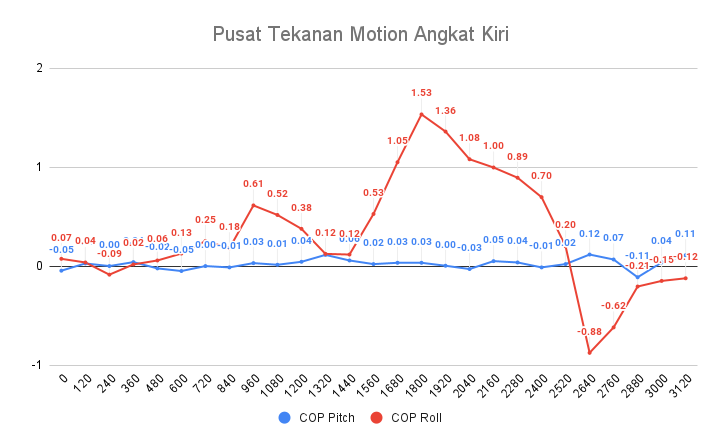
\includegraphics[width=0.45\textwidth]{gambar/Angkat_Kiri.png}
            \caption{Center of Pressure Graph When the Robot Lifts Its Left Foot}
            \label{fig:pusat_tekanan_kiri}
        \end{figure}

        \hspace*{1em} The test results show that the center of pressure dynamically changes while the robot is walking. When the robot lifts its left foot, the center of pressure shifts to the right foot, and the center pressure value on the X-axis has a minimum value of -0.5. On the Y-axis, the center pressure value ranges from -1 to 1, indicating that the center of pressure is in the middle of the sole.
\end{enumerate}
